\documentclass[14pt,a4paper,report]{report}
\usepackage[a4paper, mag=1000, left=2.5cm, right=1cm, top=2cm, bottom=2cm, headsep=0.7cm, footskip=1cm]{geometry}
\usepackage[utf8]{inputenc}
\usepackage[english,russian]{babel}
\usepackage{indentfirst}
\usepackage[dvipsnames]{xcolor}
\usepackage[colorlinks]{hyperref}
\usepackage{listings} 
\usepackage{fancyhdr}
\usepackage{caption}
\usepackage{graphicx}
\hypersetup{
	colorlinks = true,
	linkcolor  = black
}

\usepackage{titlesec}
\titleformat{\chapter}
{\Large\bfseries} % format
{}                % label
{0pt}             % sep
{\huge}           % before-code


\DeclareCaptionFont{white}{\color{white}} 

% Listing description
\usepackage{listings} 
\DeclareCaptionFormat{listing}{\colorbox{gray}{\parbox{\textwidth}{#1#2#3}}}
\captionsetup[lstlisting]{format=listing,labelfont=white,textfont=white}
\lstset{ 
	% Listing settings
	inputencoding = utf8,			
	extendedchars = \true, 
	keepspaces = true, 			  	 % Поддержка кириллицы и пробелов в комментариях
	language = C,            	 	 % Язык программирования (для подсветки)
	basicstyle = \small\sffamily, 	 % Размер и начертание шрифта для подсветки кода
	numbers = left,               	 % Где поставить нумерацию строк (слева\справа)
	numberstyle = \tiny,          	 % Размер шрифта для номеров строк
	stepnumber = 1,               	 % Размер шага между двумя номерами строк
	numbersep = 5pt,              	 % Как далеко отстоят номера строк от подсвечиваемого кода
	backgroundcolor = \color{white}, % Цвет фона подсветки - используем \usepackage{color}
	showspaces = false,           	 % Показывать или нет пробелы специальными отступами
	showstringspaces = false,    	 % Показывать или нет пробелы в строках
	showtabs = false,           	 % Показывать или нет табуляцию в строках
	frame = single,              	 % Рисовать рамку вокруг кода
	tabsize = 2,                  	 % Размер табуляции по умолчанию равен 2 пробелам
	captionpos = t,             	 % Позиция заголовка вверху [t] или внизу [b] 
	breaklines = true,           	 % Автоматически переносить строки (да\нет)
	breakatwhitespace = false,   	 % Переносить строки только если есть пробел
	escapeinside = {\%*}{*)}      	 % Если нужно добавить комментарии в коде
}

\begin{document}

\def\contentsname{Содержание}

% Titlepage
\begin{titlepage}
	\begin{center}
		\textsc{Санкт-Петербургский Политехнический 
			Университет Петра Великого\\[5mm]
			Кафедра компьютерных систем и программных технологий}
		
		\vfill
		
		\textbf{Отчёт по лабораторной работе №1\\[3mm]
			Курс: «Интеллектуальные системы»\\[41mm]
		}
	\end{center}
	
	\hfill
	\begin{minipage}{.4\textwidth}
		Выполнил студент:\\[2mm] 
		Бояркин Н.С.\\
		Группа: 13541/3\\[5mm]
		
		Проверил:\\[2mm] 
		Сазанов А.М.
	\end{minipage}
	\vfill
	\begin{center}
		Санкт-Петербург\\ \the\year\ г.
	\end{center}
\end{titlepage}

% Contents
\tableofcontents
\clearpage

\chapter{Лабораторная работа №1}

\section{Цель работы}

Научиться оформлять отчеты по лабораторным работам.

\section{Программа работы}

\begin{enumerate}
	\item Приведите развернутое определение следующих понятий: Интеллект, Ум, Разум, Мышление, Интуиция, Чувства, Инстинкт, Творчество. Что в этих понятиях общего и в чем различия? Что по вашему мнению отличает человеческое мышление от животного? Приведите
	примеры. Является ли биологический аспект (живое существо или машина) главным при принятии
	решения о разумности (интеллектуальности) объекта?
	\item Что такое интеллектуальная система? Какую систему можно назвать «по-настоящему»
	интеллектуальным? Приведите примеры «интеллектуальных» систем, и наоборот систем
	которые считаются «интеллектуальными» но по-вашему таковыми не являются.
	\item В чем отличия следующих понятий: события, факты, знания, данные?
	\item Приведите современную классификацию интеллектуальных систем и представлений знаний
	в этих системах.
	\item Перечислите и по возможности классифицируйте основные существующие системы принятия
	решения. Выявите общие черты и различия.
	\item Все ли знания могут быть формализованы? Можно ли ожидать решения задачи создания в
	полном смысле слова искусственного интеллекта? Обоснуйте свою точку зрения.
	\item Какие события, открытия, изобретения или гипотезы в области ИС наиболее перспективны по
	вашему мнению?
	\item Приведите пример ТОП-5 технологий, которые по Вашему вниманию уже сейчас активно
	меняют наш мир.
\end{enumerate}

\clearpage

\section{Ход работы}

\subsection{Задание 1}

\subsubsection{Приведите определение следующих понятий: Интеллект, Ум, Разум, Мышление, Интуиция, Чувства, Инстинкт, Творчество}

\emph{\textbf{Интеллект}} -- общие способности к познанию, пониманию и разрешению проблем. Понятие интеллект объединяет все познавательные способности индивида: ощущение, восприятие, память, представление, мышление, воображение [1]

\emph{\textbf{Ум}} -- способность думать, способность находить решение жизненных задач, способность видеть и предсказывать последствия своих действий [2]

\emph{\textbf{Разум}} -- высшая форма человеческого мышления, позволяющая отражать закономерные связи и качества вещей в рациональном знании. Проявляет себя в формах познания, целеполагания, организации, деятельности [3]

\emph{\textbf{Мышление}} -- высшая форма познавательной деятельности человека, социально обусловленный психический процесс опосредованного и обобщенного отражения действительности, процесс поисков и открытия существенно нового [4]

\emph{\textbf{Интуиция}} -- мыслительный процесс, состоящий в практически моментальном нахождении решения задачи при недостаточной осознанности логических связей [5]

\emph{\textbf{Чувства}} -- устойчивые эмоциональные переживания человека, возникающие в процессе его отношений с окружающим миром. Чувства формируются и вырабатываются в ходе развития и воспитания человека [6]

\emph{\textbf{Инстинкт}} -- форма врожденного поведения, набор определенных действий, которые возникают при совмещении внутреннего функционального состояния организма с определенными факторами окружающей среды [7]

\emph{\textbf{Творчество}} -- деятельность, результатом которой является создание новых материальных и духовных ценностей [8]

\subsubsection{Что в этих понятиях общего и в чем различия?}

Все понятия связаны друг с другом и в первую очередь ассоциируются с работой головного мозга человека. Однако, часть из этих понятий можно отнести не только к людям, но и к животным. Интеллектуальные системы, в данный момент времени, способны решать только специфические формализованные задачи, однако, при должном развитии вычислительных мощностей, возможности интеллектуальных систем приблизятся к возможностям человеческого мозга.

\subsubsection{Что по вашему мнению отличает человеческое мышление от животного? Приведите примеры}

Животное может действовать только в рамках ситуации, которая воспринимается непосредственно, а все осуществляемые им акты ограничены биологическими потребностями, то есть мотивация всегда биологическая. Конкретное, практическое мышление животных делает их зависимыми от непосредственной ситуации. Лишь в процессе ориентированного манипулирования животное способно решить проблемные задачи. Человек же благодаря абстрактному, логическому мышлению может предвидеть события, делать согласно познавательной необходимости - сознательно [9]

Отличие психики животных и человека состоит в чувствах. Животные также способны переживать положительные или отрицательные эмоции, но только человек может сочувствовать в горе или радости другому человеку, наслаждаться картинами природы, переживать интеллектуальные чувства [9]

Развитие психики в животном мире подчинено биологическим законам, а развитие психики человека детерминируется общественно-историческими условиями [9]

\subsubsection{Является ли биологический аспект главным при принятии решения о интеллектуальности объекта?}

Нет. Если полностью воссоздать человеческий мозг на электрических элементах, то сохранится вся его функциональность. Однако, ввиду чудовищных энергозатрат на вычислительные мощности, в настоящее время это невозможно.

\subsection{Задание 2}

\subsubsection{Что такое интеллектуальная система?}

\emph{\textbf{Интеллектуальная система}} -- компьютерная система, которая реализует некоторые черты человеческого интеллекта, дающие возможность осиливать трудные задачи, решение которых человеком в реальное время невозможно [10] 

\subsubsection{Какую систему можно назвать «по-настоящему» интеллектуальной?}

Которая не ограничена поставленной задачей и способна сама принимать решения.

\subsubsection{Приведите примеры «интеллектуальных» систем, и наоборот систем, которые считаются «интеллектуальными» но по-вашему таковыми не являются.}

Онлайн-переводчики, Cleverbot, Siri, FindFace и множество других. Все эти системы являются интеллектуальными.

Если система использует детерминированный алгоритм, не требующий обучения, то такая система не является интеллектуальной.

\subsection{Задание 3}

\subsubsection{В чем отличия следующих понятий: события, факты, знания, данные?}

\emph{\textbf{Событие}} -- то, что имеет место, происходит, наступает в произвольной точке пространства-времени; значительное происшествие, явление или иная деятельность как факт общественной или личной жизни; множество исходов эксперимента [11]

\emph{\textbf{Факт}} -- называется утверждение, информационное сообщение и т. д., которые отражают действительность, являются правдивыми [12]

\emph{\textbf{Знание}} -- результат познавательной деятельности человека [13]

\emph{\textbf{Данные}} -- факты и характеризующие их числовые, количественные показатели: имена, даты событий, сведения об экономических процессах, местах действия [14]

\subsection{Задание 4}

\subsubsection{Приведите современную классификацию интеллектуальных систем и представлений знаний в этих системах}

\begin{figure}[h!]
	\centering
	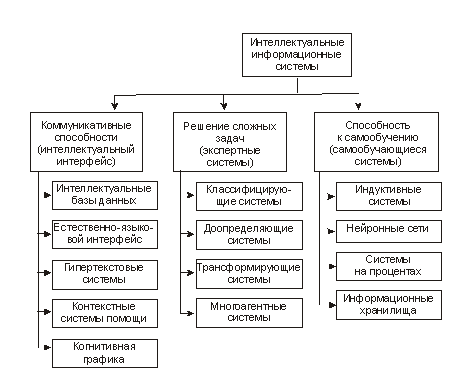
\includegraphics[scale = 1.40]{images/iis.png}
	\caption{Классификация ИИС [15]}
	\label{image:1}
\end{figure}	


\subsection{Задание 5}

\subsubsection{Перечислите и по возможности классифицируйте основные существующие системы принятия решения. Выявите общие черты и различия}

По взаимодействию с пользователем выделяют три вида СППР [16]:

\begin{itemize}
	\item пассивные помогают в процессе принятия решений, но не могут выдвинуть конкретного предложения;
	\item активные непосредственно участвуют в разработке правильного решения;
	\item кооперативные предполагают взаимодействие СППР с пользователем. Выдвинутое системой предложение пользователь может доработать, усовершенствовать, а затем отправить обратно в систему для проверки. После этого предложение вновь представляется пользователю, и так до тех пор, пока он не одобрит решение.
\end{itemize}

По способу поддержки различают [16]:

\begin{itemize}
	\item модельно-ориентированные СППР, используют в работе доступ к статистическим, финансовым или иным моделям;
	\item СППР, основанные на коммуникациях, поддерживают работу двух и более пользователей, занимающихся общей задачей;
	\item СППР, ориентированные на данные, имеют доступ к временным рядам организации. Они используют в работе не только внутренние, но и внешние данные;
	\item СППР, ориентированные на документы, манипулируют неструктурированной информацией, заключенной в различных электронных форматах;
	\item СППР, ориентированные на знания, предоставляют специализированные решения проблем, основанные на фактах.
\end{itemize}	
	
По сфере использования выделяют [16]:

\begin{itemize}
	\item общесистемные;
	\item настольные СППР.
\end{itemize}

Общесистемные работают с большими СХД и применяются многими пользователями. Настольные являются небольшими системами и подходят для управления с персонального компьютера одного пользователя [16]

\subsection{Задание 6}

\subsubsection{Все ли знания могут быть формализованы?}

Формализация знаний является потребностью человеческого общества. Формализованные знания намного проще хранить или обмениваться ими. Однако, не все знания могут быть формализованы, по крайней мере усилиями самого человека. Формализуемый накопленный опыт человека составляет всего 1-2\%, все остальное может быть изучено и интерпретировано только внешними устройствами и только в далеком будущем.

\subsubsection{Можно ли ожидать решения задачи создания в полном смысле слова искусственного интеллекта? Обоснуйте свою точку зрения.}

Все зависит от успехов в области изучения человеческого мозга, а также от изобретения высокоэффективных вычислительных систем, которые в порядки раз превосходят текущие вычислительные мощности. При соблюдении этих условий ИИ точно будет создан, как симуляция человеческого мозга.

\subsection{Задание 7}

\subsubsection{Какие события, открытия, изобретения или гипотезы в области ИС наиболее перспективны по вашему мнению?}

В ближайшем будущем успехи в области перевода текстов на различные языки полностью изменят мир. Уже сейчас успешно эксплуатируется нейронная сеть Google Neural Machine Translation System (NMTS), которая не только анализирует существующие варианты перевода в процессе обучения, но и выполняет интеллектуальный анализ предложений, разбивая их на «словарные сегменты». В определённой репрезентации внутри сети эти «словарные сегменты» соответствуют смыслам слов. По сравнению с машинным переводом, качество сильно улучшилось, в некоторых случаях достигая качества человеческого перевода [17]

Если объединить эту функциональность с успехами в области распознавания речевых команд, то устройства для качественного перевода речи в реальном времени не заставят себя ждать, практически полностью стерев границы между национальностями.

\subsection{Задание 8}

\subsubsection{Приведите пример ТОП-5 технологий, которые по Вашему вниманию уже сейчас активно меняют наш мир.}

\begin{itemize}
	\item Переводчики.
	\item Распознавание лиц, отпечатков пальцев.
	\item Распознавание документов.
	\item Распознавание речевых команд.
	\item Ассоциативный поиск и фильтрация спама.
\end{itemize}

\section{Вывод}

В рамках данной работы были выявлены основные области нашей жизни, в которых применяются ИС. Кроме того были проведены аналогии ИС с человеческим мозгом и определены основные проблемы создания ИИ.

\clearpage

\section{Список литературы}

% [16] https://geektimes.ru/post/280912/

% \linebreak

\begin{flushleft}

[1] Интеллект человека: определение, особенности и виды интеллекта [Электронный ресурс]. — URL: \href{http://www.grandars.ru/college/psihologiya/intellekt-cheloveka.html}{http://www.grandars.ru/college/psihologiya/intellekt-cheloveka.html} (дата обращения 16.09.2017).

[2] Что такое - ум? [Электронный ресурс]. — URL: \href{http://www.psychologos.ru/articles/view/chto-takoe---um-vop-zn--kto-takoy---umnyy-chelovek-vop-zn-}{http://www.psychologos.ru/articles/view/chto-takoe---um-vop-zn--kto-takoy---umnyy-chelovek-vop-zn-} (дата обращения 16.09.2017).

[3] РАЗУМ это что такое РАЗУМ: определение — Философия.НЭС [Электронный ресурс]. — URL: \href{http://terme.ru/termin/razum.html}{http://terme.ru/termin/razum.html} (дата обращения 16.09.2017).

[4] Мышление – как познавательный процесс [Электронный ресурс]. — URL: \href{http://www.no-stress.ru/Uchebniki/general-psych/myshlenie.html}{http://www.no-stress.ru/Uchebniki/general-psych/myshlenie.html} (дата обращения 16.09.2017).

[5] Интуиция. Что такое "Интуиция"? [Электронный ресурс]. — URL: \href{http://www.psychologies.ru/glossary/09/intuitsiya/}{http://www.psychologies.ru/glossary/09/intuitsiya/} (дата обращения 16.09.2017).

[6] Чувства. Что такое "Чувства"? [Электронный ресурс]. — URL: \href{http://www.psychologies.ru/glossary/23/chuvstva/}{http://www.psychologies.ru/glossary/23/chuvstva/} (дата обращения 16.09.2017).

[7] Инстинкт - Психологос [Электронный ресурс]. — URL: \href{http://www.psychologos.ru/articles/view/instinkt}{http://www.psychologos.ru/articles/view/instinkt} (дата обращения 16.09.2017).

[8] Что такое Творчество, значение, словарь, энциклопедия [Электронный ресурс]. — URL: \href{http://www.insai.ru/slovar/tvorchestvo}{http://www.insai.ru/slovar/tvorchestvo} (дата обращения 16.09.2017).

[9] Чем отличается сознание человека от сознания животного? [Электронный ресурс]. — URL: \href{https://thequestion.ru/questions/139727/chem-otlichaetsya-soznanie-cheloveka-ot-soznaniya-zhivotnogo}{https://thequestion.ru/questions/139727/chem-otlichaetsya-soznanie-cheloveka-ot-soznaniya-zhivotnogo} (дата обращения 16.09.2017).

[10] Что такое интеллектуальные системы? [Электронный ресурс]. — URL: \href{http://epistemology\_of\_science.academic.ru/253/\%D0\%B8\%D0\%BD\%D1\%82\%D0\%B5\%D0\%BB\%D0\%BB\%D0\%B5\%D0\%BA\%D1\%82\%D1\%83\%D0\%B0\%D0\%BB\%D1\%8C\%D0\%BD\%D1\%8B\%D0\%B5\_\%D1\%81\%D0\%B8\%D1\%81\%D1\%82\%D0\%B5\%D0\%BC\%D1\%8B}{http://epistemology\_of\_science.academic.ru/253/интеллектуальные\_системы} (дата обращения 16.09.2017).

[11] Событие - Психологос [Электронный ресурс]. — URL: \href{http://www.psychologos.ru/articles/view/sobytie}{http://www.psychologos.ru/articles/view/sobytie} (дата обращения 16.09.2017).

[12] Что такое факт? [Электронный ресурс]. — URL: \href{http://dic.academic.ru/dic.nsf/dmitriev/5687\%D1\%84\%D0\%B0\%D0\%BA\%D1\%82}{http://dic.academic.ru/dic.nsf/dmitriev/5687/факт} (дата обращения 16.09.2017).

[13] Знание - определение [Электронный ресурс]. — URL: \href{psihotesti.ru/gloss/tag/znanie/}{psihotesti.ru/gloss/tag/znanie/} (дата обращения 16.09.2017).

[14] ДАННЫЕ — определение термина [Электронный ресурс]. — URL: \href{https://tochka.com/info/glossary/\%D0\%94\%D0\%90\%D0\%9D\%D0\%9D\%D0\%AB\%D0\%95}{https://tochka.com/info/glossary/ДАННЫЕ} (дата обращения 16.09.2017).

[15] ВГУЭС. Информационные технологии в экономике [Электронный ресурс]. — URL: \href{https://abc.vvsu.ru/books/up_inform_tehnol_v_ekon/page0017.asp}{https://abc.vvsu.ru/books/up\_inform\_tehnol\_v\_ekon/page0017.asp} (дата обращения 16.09.2017).

[16] Переводчик Google Translate подключили к нейросети [Электронный ресурс]. — URL: \href{https://geektimes.ru/post/280912/}{https://geektimes.ru/post/280912/} (дата обращения 16.09.2017).

\end{flushleft}
	


\end{document}